\subsection{Glyph: \glyph{And}}
\label{sec:af:and}

The glyph \glyph{and} is used to denote that all the \glyph{ANs} linked as input are necessary to influence the target activity.

\begin{glyphDescription}
 \glyphSboTerm SBO:0000173 ! and.
 \glyphIncoming One or more \glyph{logic arcs} (\sect{af:logicArc}).
 \glyphOutgoing  One \glyph{logic arc} (\sect{af:logicArc}) or one of the modulation arcs (\sect{af:arcs}).
 \glyphContainer An \glyph{and} operator is represented by a circular shape containing the word ``AND''.
The shape is linked to two ports, that are small arcs attached to the centres of opposite sides of the shape, as shown in \fig{af:and}.
The incoming \glyph{logic arcs} (\sect{af:logicArc}) are linked to the extremity of the leftmost or uppermost port, while the outgoing \glyph{logic arc} (\sect{af:logicArc}) or modulation arc (\sect{af:arcs}) is linked to the extremity of the rightmost or bottommost port.
 \glyphLabel None.
 \glyphAux None.
\end{glyphDescription}

\begin{figure}[H]
  \centering
  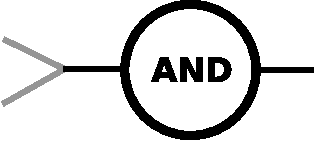
\includegraphics[scale = 1]{images/build/and.pdf}
  \caption{The \AF glyph for \glyph{and}. Only two inputs are represented, but more would be allowed.}
  \label{fig:af:and}
\end{figure}
